\documentclass[10pt]{article}
\usepackage{amsmath}
\usepackage{mathtools}
\DeclarePairedDelimiter{\abs}{\lvert}{\rvert}
\usepackage[hidelinks]{hyperref}
\usepackage{amssymb}
\usepackage{tikz}
\usepackage{caption}
\usepackage{graphicx}
\usepackage[T1]{fontenc}
\graphicspath{{.}}
\usepackage{listings}
\usepackage{verbatim}
\usepackage{subfigure}
\lstset{
language=[LaTeX]TeX,
backgroundcolor=\color{gray!25},
basicstyle=\ttfamily,
columns=flexible,
breaklines=true
}
\captionsetup{labelsep=space,justification=justified,singlelinecheck=off}
\reversemarginpar
\usepackage[paper=a4paper,
            %includefoot, % Uncomment to put page number above margin
            marginparwidth=10mm,      % Length of section titles
            marginparsep=0.8mm,       % Space between titles and text
            margin=10mm,              % 25mm margins
            includemp]{geometry}

\begin{document}
\section*{}
\begin{flushleft}
Name: Krishna Chaitanya Sripada\\
\end{flushleft}
\section*{Analysis: }
\begin{flushleft}
(a) Since we need to train the classifier to distinguish 3's from 8's, we use the MNIST training data to fit the SVC and then use the MNIST test data to predict the labels for the test samples. Both the training and the test data contain data corresponding to 3's and 8's. The training data was fit to the SVC using a ``linear'' kernel and then the test data was used to predict the labels of the samples. This returned an accuracy of 0.968. The training data was also fit to the SVC using a ``rbf'' kernel and then the test data was used to predict the labels of the samples. This returned an accuracy of 0.969. The results are shown below:\\
\begin{figure}[!htp]
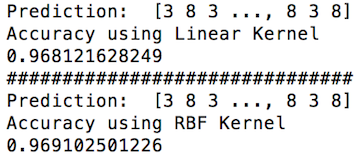
\includegraphics{result1.png}
\caption{:Result of SVM Classification with Linear and RBF Kernels}
\end{figure}
\vspace{0.5em}
(b) The values of the regularization parameter ``C'' that were tested are [0.1, 0.01, 0.001, 0.0001, 1, 2, 5, 10, 100] and ``linear'' and ``rbf'' kernels were used to fit the data. The results are shown below:\\
\begin{figure}[!htp]
	\subfigure[Linear and RBF Kernels with C=0.1, 0.01, 0.001, 0.001]{
		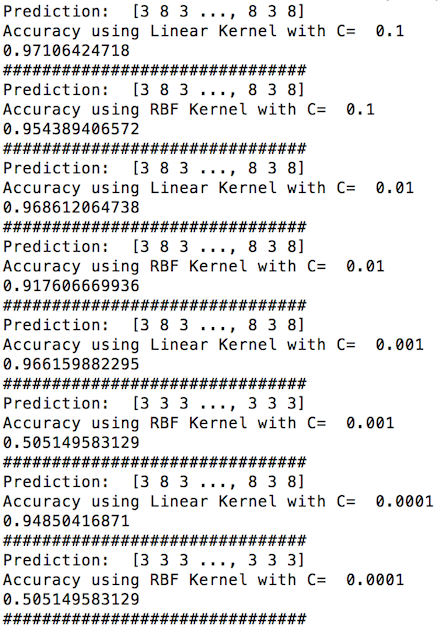
\includegraphics[width=4cm]{result2.png}}
	\subfigure[Linear and RBF Kernels with C=1, 2, 5, 10, 100]{
		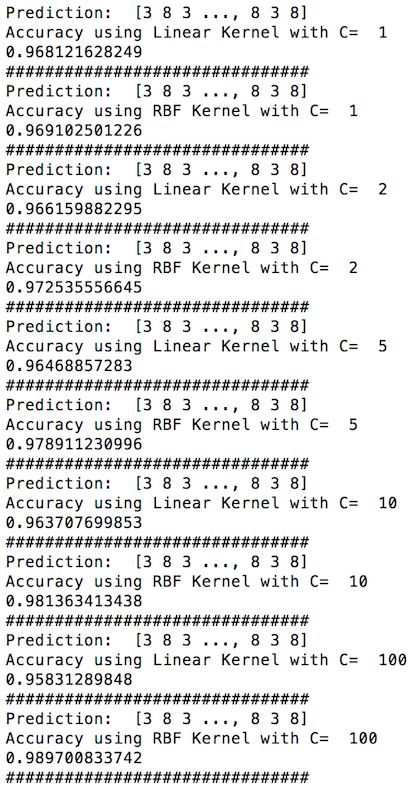
\includegraphics[width=4cm]{result3.png}}
	\caption{:Linear and RBF kernels with different regularization parameter ``C'' values}
	\label{fig: Linear and RBF kernels with different regularization parameter ``C'' values}
\end{figure}
\vspace{0.5em}
(c) Examples of support vectors are shown below:\\
\begin{figure}[!htp]
	\subfigure[Support Vector `8']{
		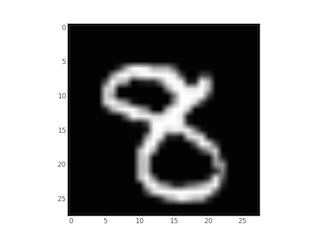
\includegraphics[width=4cm]{result4.png}}
	\subfigure[Support Vector `3']{
		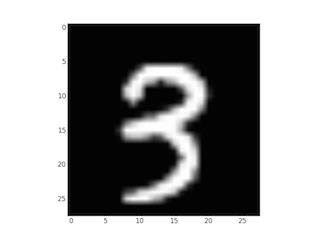
\includegraphics[width=4cm]{result5.png}}
	\caption{:Examples of Support Vectors}
	\label{fig: Examples of Support Vectors}
\end{figure}
\end{flushleft}
\end{document}